\chapter{Implementasi dan Pengujian}
\label{chap:implementasidanpengujian}

Bab ini membahas mengenai implementasi dan pengujian perangkat lunak SharIF Judge.

\section{Lingkungan Implementasi dan Pengujian}
\label{sec:5:lingkungan}

Implementasi perangkat lunak dilakukan pada perangkat penulis dengan spesifikasi sebagai berikut:

\begin{itemize}
    \item Perangkat Keras:
    \begin{itemize}
        \item \textit{Processor}: Intel Core i5-7600
        \item \textit{Random Access Memory}: 16GB DDR4
        \item \textit{Storage}: 500GB SSD dan 2TB HDD
    \end{itemize}
        \item Perangkat Lunak:
    \begin{itemize}
        \item \textit{Operating System}: Windows 10 Home 64-bit
        \item \textit{Windows Subsystem for Linux}: Ubuntu 20.04.2 LTS
    \end{itemize}
\end{itemize}

\section{Implementasi}
\label{sec:5:implementasi}

\subsection{Tampilan Antarmuka}
\label{subsec:5:antarmuka}

\begin{figure}[H]
	\centering  
	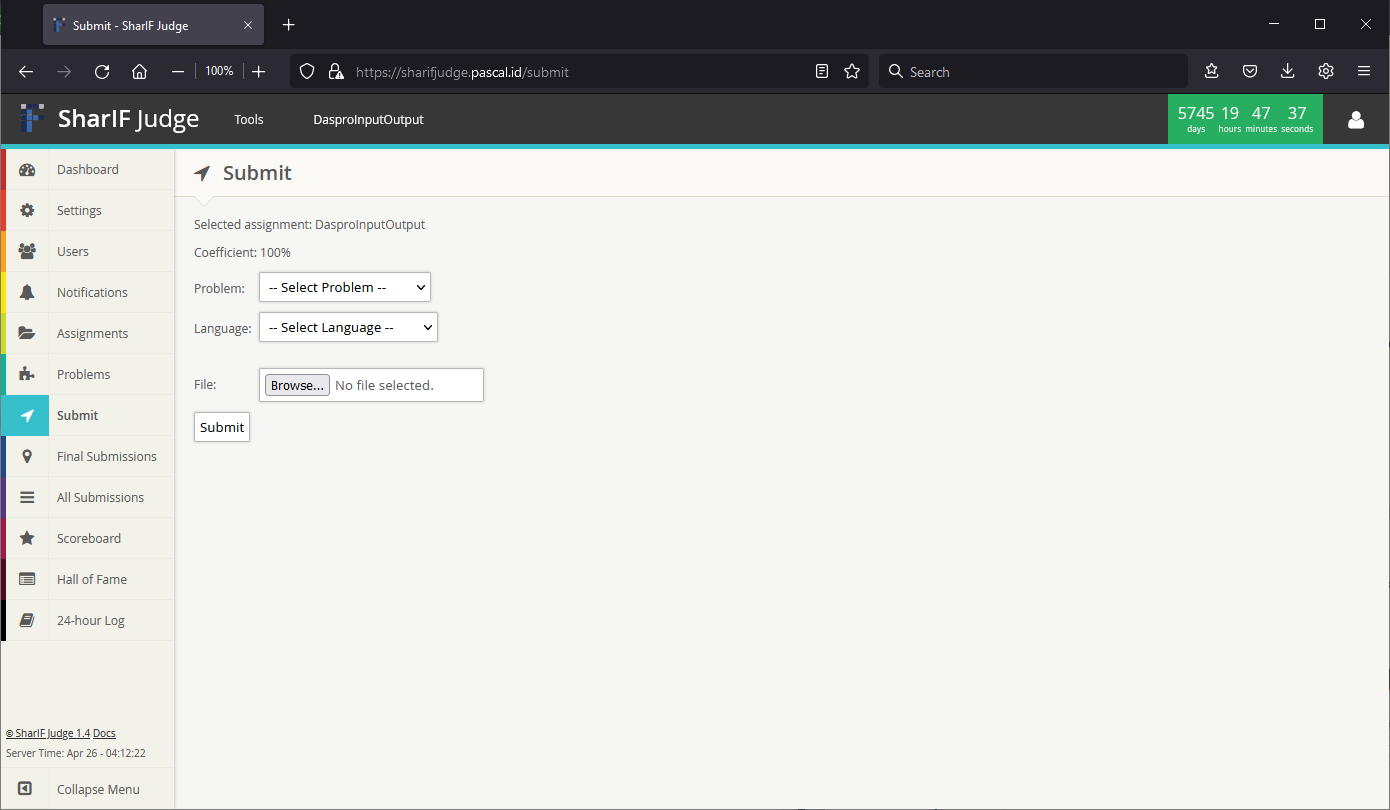
\includegraphics[scale=0.35]{submit}  
	\caption{Antarmuka halaman Submit} 
	\label{fig:5:antarmuka} 
\end{figure}

Gambar \ref{fig:5:antarmuka} merupakan antarmuka pada halaman Submit yang sudah diimplementasikan. Seluruh perubahan tampilan diimplementasikan pada \textit{view} \verb|submit.twig|, beserta dengan \textit{stylesheet} yang terdapat di \verb|application\views\pages\submit.twig| dan \textit{script} pada \verb|assets\js\shj_submit.js|.

\subsection{Menampilkan soal}
\label{subsec:5:soal}

\begin{lstlisting}[language=php, caption=Penambahan \texttt{iframe} untuk PDF.js, label=kode:5:pdfjs]
    <iframe id="pdf_viewer" src={{ base_url('assets/pdfjs/web/viewer.html?file=') ~ site_url('assignments/pdf/' ~ user.selected_assignment.id ~ '/null/true')}} ></iframe>
\end{lstlisting}


\section{Pengujian}
\label{sec:5:pengujian}

\subsection{Pengujian Fungsional}
\label{subsec:5:fungsional}

Pengujian fungsional dilakukan secara lokal pada perangkat penulis. Berikut ini pengujian yang dilakukan terhadap fitur-fitur yang sudah diimplementasi:


\subsection{Pengujian Eksperimental}
\label{subsec:5:eksperimental}

Pengujian eksperimental dilakukan pada mata kuliah Dasar-dasar Pemrograman semester 51 Teknik Informatika Unpar. Perangkat lunak diuji pada \textit{judge} dengan alamat \verb|http://daspro.labftis.net|. Seluruh persoalan dan masukan yang diterima selama mata kuliah Dasar-dasar Pemrograman dicatat pada \verb|https://github.com/athlonneo/SharIF-Judge/issues|.



